\chapter{Data Structure Optimisation and Software Architecture Design for the Implementation of Large-Scale Spiking Neural Networks}
\label{chap:large_snn}
\section{Introduction}
Chapters \ref{chap:snn} and \ref{chap:neucube} have, on numerous occasions, discussed the importance of finding a trade-off between the biological plausibility and the computational complexity of computational models. The discussions have, especially, been focused on the spiking neuron. In this Chapter, the concentration will be on implementation level design considerations for simulating scalable spiking neural network architectures. The push towards big data analytics is driving the development of fast, scalable and real-time pattern recognition systems all over the world. Scalability of the machine learning framework plays a crucial role in realising the big data dream. Interestingly, this issue of scalability was seldom solved using actual scaling in machine learning, at least not in the big data sense. Part of the reason is certainly that multi-core processors did not yet exist on the scale they do today and that the idea of “just scaling out” was not as pervasive as it is today. Instead, `scalable' machine learning is almost always based on finding more efficient algorithms, and most often, approximations to the original algorithm which can be computed much more efficiently. According to Vowpal Wabbit \citep{langford2007vowpal}:

\emph{"There are two ways to have a fast learning algorithm: (a) start with a slow algorithm and speed it up, or (b) build an intrinsically fast learning algorithm. This project is about approach (b), and it’s reached a state where it may be useful to others as a platform for research and experimentation."}

This Chapter will be taking the first approach and will use the second layer or the SNNc component of the NeuCube framework (Read Chapter \ref{chap:neucube} for overview) to drive the discussion. Before moving into the crux of this Chapter, a broad picture of the contrasting properties of a digital computer will be painted. There will also be discussions of a biological brain which poses significant challenges in integrating both in a single framework.
\section{Brain vs. Digital Computers}
 Although, the brain-computer metaphor has served cognitive psychology well, research in cognitive neuroscience has revealed many important differences between brains and computers.
\begin{enumerate}
	\item Memory and storage: In computers, data stored in memory is accessed by looking at a precise memory location. This is known as byte-address memory. On the contrary, the brain uses content-address memory, such that data can be addressed in memory through activation spread from closely related concepts.
	
	\item Parallelism: The brain is naturally a massively parallel machine. Communication and synchronisations are automatically dealt with by the neuronal mesh of the brain. On the other hand, von Neumann architecture driven computer systems are modular and serial. Parallelism cannot be integrated into such an architecture intuitively.
	
	\item Processing speed and system clock: The speed of neural information processing is subject to a variety of constraints, including the time for electrochemical signals to traverse axons and dendrites, axonal myelination, the diffusion time of neurotransmitters across the synaptic cleft, differences in synaptic efficacy, the coherence of neural firing, the current availability of neurotransmitters, and the prior history of neuronal firing. Although there are individual differences in processing speed, this does not reflect a monolithic or unitary construct, and certainly nothing as concrete as the speed of a microprocessor. Instead, psychometric “processing speed” probably indexes a heterogeneous combination of all the speed constraints mentioned above. Similarly, there does not appear to be any central clock in the brain, and there is debate as to how clock-like the brain’s time-keeping devices actually are.
	
	\item Processing unit and memory interactions: Computers process information from memory using CPUs, and then write the results of that processing back to memory. No such distinction exists in the brain. As neurons process information they are also modifying their synapses which are themselves the substrate of memory. 
	
	\item Heterogeneity and size: The brain in its full maturity is a gigantic network of over $86$ billion brain cells (or neurons) with approximately $1750$ synapses per neuron. It is estimated that a truly biological model of the brain would have to include nearly $225$ million billion interactions between cell types, neuro-transmitters, neuro-modulators, axonal branches and dendritic spines. This means layers of hierarchy and heterogeneity is present in the brain with complex interactions among them. 
\end{enumerate} 

\section{NeuCube SNNc}
The second layer or the SNNc layer of the NeuCube (see \figurename \ref{fig:neucube_archit}) is considered to be the most complex layer of the NeuCube architecture and it is computationally most expensive. For example, the NeuCube implementation distributed as part of the prototyping and testing module requires gigabyte order memory for running the unsupervised learning for an SNNc of size less than $1000$ neurons. Hence, it is necessary to concentrate on this layer to improve scalability of the NeuCube system. 

\subsection{SNNc Architecture, Mapping and Initialisation Scheme}
\label{subsec:SNNc_init}
The SNNc architecture of NeuCube consists of a spatially arranged (in three dimensions) set of neurons (computational units), denoted by set $M$ (with $|M|$ defining the cardinality of the set). The neurons are partially connected by recurrent synapses forming a directed incomplete and acyclic graph. The neurons and synapses form the vertices and the edges of the graph. The SNNc architecture is thus formalised as a directed graph $G=\{M, C, W\}$, consisting of the set of neurons $M$, the set of directed synaptic connections, $C$ and the corresponding strengths or weights of the connections $W$. The network consists of two types of neuron: 
\begin{itemize}
	\item Input neurons: The input neurons, denoted by set $N\subset M$ (with $|N|$ defining the cardinality of the set), feed the input spike data (generated by the encoding layer) to the SNNc. These neurons do not have any activations and do not perform any computations. The input neurons form a similar level of abstraction as does the input layer in traditional neural networks. It is apparent that the input neurons do not have pre-synaptic connections, \emph{i.e.}, a synapse can only originate from such a neuron.  
	\item Spiking neurons: The spiking neurons, denoted by set $Q\subset M$ (with $|Q|$ defining the cardinality of the set), are the computational units, and are leaky integrate and fire (LIF) in nature. These neurons are responsible for performing computations on input data. The details of the neuron model is described later. These neurons can act both as post and pre-synaptic (connection) neurons, \emph{i.e.} if one considers a pair of neurons connected by a directed synapse, the synapse can both originate and end at a spiking neuron.
\end{itemize} 
The neurons in the SNNc are arranged spatially following the natural spatial arrangements in the data or by using automated mapping algorithms. \citet{tu2017mapping} maps feature covariance in the data to Euclidean distance in the SNNc. The spatial arrangement of the neurons are typically done in two or three dimensional space. The synaptic connectivity of the SNNc graph is created using the small world connectivity (SWC) algorithm \citep{kasabov2014evolving, tu2014neucube}. The SWC algorithm connects a neuron to its spatial neighbourhood (controlled by the hyperparameter radial distance $r_{swc}$) of neurons.   

\subsection{Neuron Dynamics Model}
\label{subsec:SNNc_neuron_model}

The activation of the spiking neurons present in the SNNc is modelled by the spike response model (SRM), which is a kernel based simplified realisation of the LIF model. The SRM model generalises the differential equation based dynamics of the LIF model (see \equationname \ref{eq:if_4}) by replacing them with arbitrary kernels. SRM is a powerful computational framework for temporal integration with elegant mathematical formulation.

\figurename \ref{fig:neuron_architecture} shows a typical example of a spiking neuron's configuration. A spiking neuron has a multi-input, multi-output configuration. A pair of neurons are connected by synapses. The synaptic strengths are represented by $\mathbf{w_i}$. A spiking neuron receives spike data at different time instances from the pre-synaptic neurons and emit spike data when sufficiently stimulated. The activation state of a spiking neuron $i$ is described by the membrane potential $v_i$. In a non-stimulated state, the membrane potential is said to be in a resting state $v_{rest}=0$. The SRM model in the present setup consists of multiple components:

\subsubsection{Post-synaptic Potential Kernel}
Firing of pre-synaptic neuron $j$ at time $t_j^f$, evokes a post-synaptic potential (PSP) in neuron $i$ and is modelled by the kernel response function $\epsilon_0$. 

\begin{equation}
\epsilon_0=\exp(-\frac{t-t_j^f}{\tau_m})\mathcal{H}(t-t_j^f)
\label{eq:PSP}
\end{equation}
where 

\begin{equation}
\mathcal{H}(t-t_j^f)=\left\{
\begin{array}{@{}ll@{}}
1, & \text{if}\ t-t_j^f\geq 0 \\
0, & \text{otherwise}
\end{array}\right.
\end{equation}

The PSP kernel is a function of $t-t_j^f$, representing the PSP trace over time generated by the firing of neuron $j$ over time. \figurename \ref{fig:PSP} plots the PSP kernel as the function of $t-t^f$. $\tau_m$ (\equationname \ref{eq:PSP}) is the membrane constant which controls the decay rate of the PSP. 
\begin{figure}
	\centering
	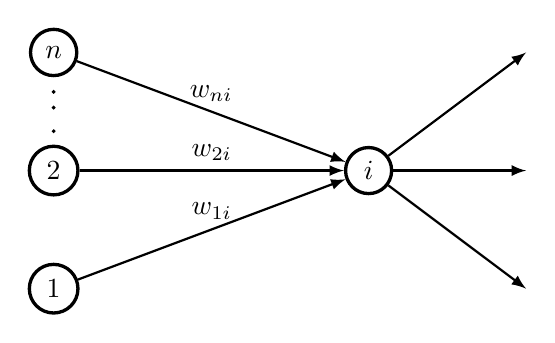
\begin{tikzpicture}
	
	\tikzstyle{connect}=[-latex, thick]
	
	\node[draw, shape=circle, very thick] (i) at (2, 0.5) {$i$};
	\node[draw, shape=circle, very thick]  (j1) at (-2, -1) {$1$};
	\node[draw, shape=circle, very thick]  (j2) at (-2, 0.5) {$2$};
	\node[draw, shape=circle, very thick]  (jk) at (-2, 2) {$n$};
	\node[draw, shape=circle, fill, scale=0.1] (d1) at (-2, 1) {};
	\node[draw, shape=circle, fill, scale=0.1] (d2) at (-2, 1.3) {};
	\node[draw, shape=circle, fill, scale=0.1] (d3) at (-2, 1.5) {};
	\coordinate (x1) at (4,-1); 
	\coordinate (x2) at (4,0.5);
	\coordinate (x3) at (4,2);
	
	
	\draw 	(jk) edge[connect] node[above]{$w_{ni}$} (i) 
	(d1)
	(d2)
	(d3)
	(j2) edge[connect] node[above]{$w_{2i}$} (i) 
	(j1) edge[connect] node[above]{$w_{1i}$} (i)
	(i) edge[connect] (x1)
	(i) edge[connect] (x2)
	(i) edge[connect] (x3);
	\end{tikzpicture}
	\caption{A typical connectivity configuration of a spiking neuron $i$.}
	\label{fig:neuron_architecture}
\end{figure}

\begin{figure}
	\centering
	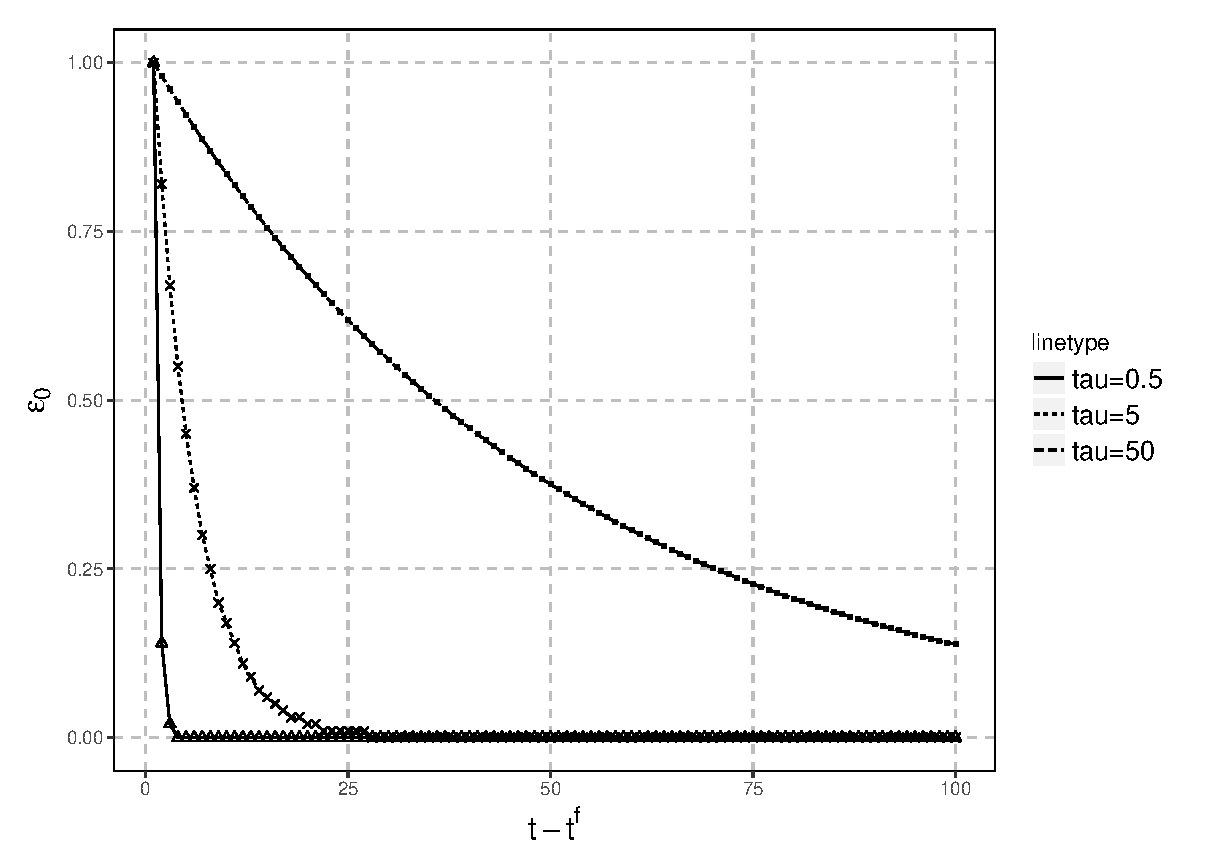
\includegraphics[width=0.8\textwidth]{fig/fmridti/potential_kernel.eps}
	\caption{Plot of the PSP trace $\epsilon_0$ as a function of $t-t^f$. This figure plots the PSP simulation for different $\tau_m$.}
	\label{fig:PSP}
\end{figure}




\subsubsection{Temporal Integration of PSP Kernels and Conditions for Spike Emission}
Under the SRM model, the PSPs evoked by the pre-synaptic neurons are temporally integrated to activate the spiking neuron. The overall contribution of the pre-synaptic spikes elicited by the pre-synaptic neurons $j$ at any time $t$ is given as \equationname \ref{eq:SRM0} describing the SRM model:


\begin{equation}
v_i(t)=v_{rest}+\sum_{j\in \Tau_i }w_{ji}\sum_{t_j^f\in F_j}\epsilon_0(t-t_j^f)
\label{eq:SRM0}
\end{equation}

The temporal summation is a double summation operation. The inner sum adds up the PSP contributions due to the firings $t_j^f\in F_j$ of one pre-synaptic neuron. The outer sum adds up the PSP contributions of all the pre-synaptic neurons $j\in \mathcal{T}_i$ connected to neuron $i$. \equationname \ref{eq:SRM0} describes the membrane potential (activation state) $v_i$ of a spiking neuron $i$ can be calculated by adding the resting potential term and the temporal PSP sum. Each incoming spike perturbs the value of $v_i$ and if, after the summation of the inputs, the membrane potential reaches the threshold $v_{thr}$ then an output spike is generated. The firing time is given by the condition $v_i(t_i^f)>=v_{thr}$. After a neuron fires the neurons' membrane potential is reset to $v_{rest}$. In standard NeuCube implementations, the inner sum is generally set to $1$. By setting the inner sum to $1$, NeuCube only uses the information of present instance and forgets the influence of historical spike-trains, thus demonstrating minimal memory in the neuron model. However, any instance of the usage of NeuCube based architecture in this thesis uses the historical information with a preset hyperparameter controlling the memory horizon.   

\subsubsection{Refractory Period}
After emitting the spike, a spiking neuron enters a period of quietness known as the refractory period. During this period, the membrane potential remains unaffected by incoming spikes. The refractory behaviour can be mathematically achieved by setting the membrane potential to a infinitely low value. In the SRM model the neuron behaviour under the influence of refractoriness depends only on the last firing moment leading to a short-term memory in the neuron. In the literature, the refractory period is described by absolute and relative refractory period. During the absolute refractory period, the neurons do not accumulate membrane potential and hence cannot fire. During the relative refractory period, it can be relatively difficult but not impossible to fire the neuron. In this current implementation, an absolute refractory period for the sake of simplicity has been used here. The absolute refractory period of a neuron is specified by the hyperparameter $\eta_{thr}$. 

The modified SRM neuronal dynamics of NeuCube is formalised by \equationname \ref{eq:SRM_neucube}. The modifications of the canonical SRM model can be observed in: (1) the implementation of the PSP kernel which outputs a unit pulse at the time neuron $i$ receives a spike from neuron $j$; (2) the implementation of refractoriness, where the membrane potential is set to negative infinity during the period $\eta_{thr}$ after neuron $i$ fires a spike at time $t_i^f$.
\begin{equation}
\begin{matrix}
\displaystyle v_i(t)=v_{rest}+\sum_{j\in \Tau_i }w_{ji}\sum_{t_j^f\in F_j}\epsilon_0(t-t_j^f)+\eta(t-t_i^f) \\

\epsilon_0(t-t_j^f)=\left\{
\begin{array}{@{}cc@{}}
1, & \text{if}\ t-t_j^f=0 \\
0, & \text{otherwise}
\end{array}\right. \\

\eta(t-t_i)=\left\{
\begin{array}{@{}cc@{}}
-\infty, & \text{if}\ t-t_i^f<\eta_{thr}\\
0, & \text{otherwise}
\end{array}\right.

\end{matrix}
\label{eq:SRM_neucube}
\end{equation}

\begin{figure}
	\centering
	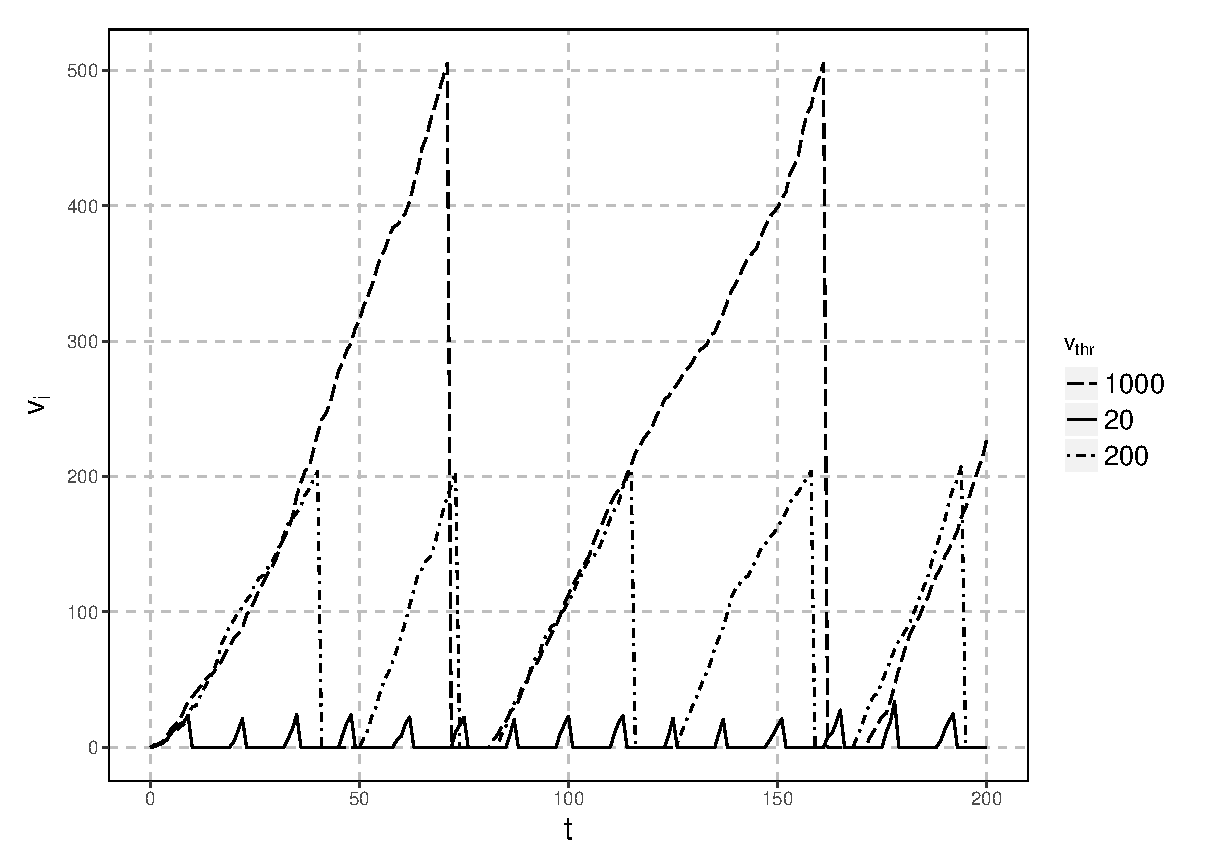
\includegraphics[width=0.8\linewidth]{fig/fmridti/membrane_potential.eps}
	\caption{Plot of the membrane potential traces($v_i$) of a neuron $i$ simulated over $T=200$ time points using the SRM model. For the simulations, $3$ predecessor neurons were connected to a spiking neuron. The spike data from the predecessor neurons are sampled randomly from uniform random distribution. The $\eta_{thr}$ for the spiking neuron was set to $10$. Each of the three $v_i$ traces correspond to a preset $v_{thr}$ mentioned in the label.}
	\label{fig:SRM}
\end{figure}

\figurename \ref{fig:SRM} shows a plot of three simulations of a spiking neuron for $200$ discrete times with random spike inputs. Each simulation uses a preset $v_{thr}$. At the beginning of the simulation, the neuron is in a resting state $v_{t=0}=v_{rest}$. With the arrival of spikes, the membrane potential increases in a linear fashion and when sufficiently stimulated (sufficiency is determined by $v_{thr}$), the neuron spikes, and then goes back to the resting state. At this point, the neuron is said to be in a refractory state. The neuron stays in this state for a predetermined period $\eta_{thr}$ and then goes back to a non-refractory state.  

\subsection{Unsupervised Weight Adaptation in SNNc}

The unsupervised weight adaptation mechanism in the SNNc is an extremely important aspect of the dynamics. In a neural network paradigm, learning or plasticity is achieved through the synaptic strength updates of the network. The learning behaviour of the SNNc can be explained using the learning model of a single spiking neuron. Considering the single neuron architecture in \figurename \ref{fig:neuron_architecture}, the unsupervised learning problem is to formalise a scheme of updating the weights $W$ of the network by $\Delta W(t)$ over the simulation time $T$. The NeuCube SNNc has employed numerous variations of temporally asynchronous forms of Hebbian learning in different implementations. 

\subsubsection{STDP} 
\label{subsec:STDP}
\begin{figure}
	\centering
	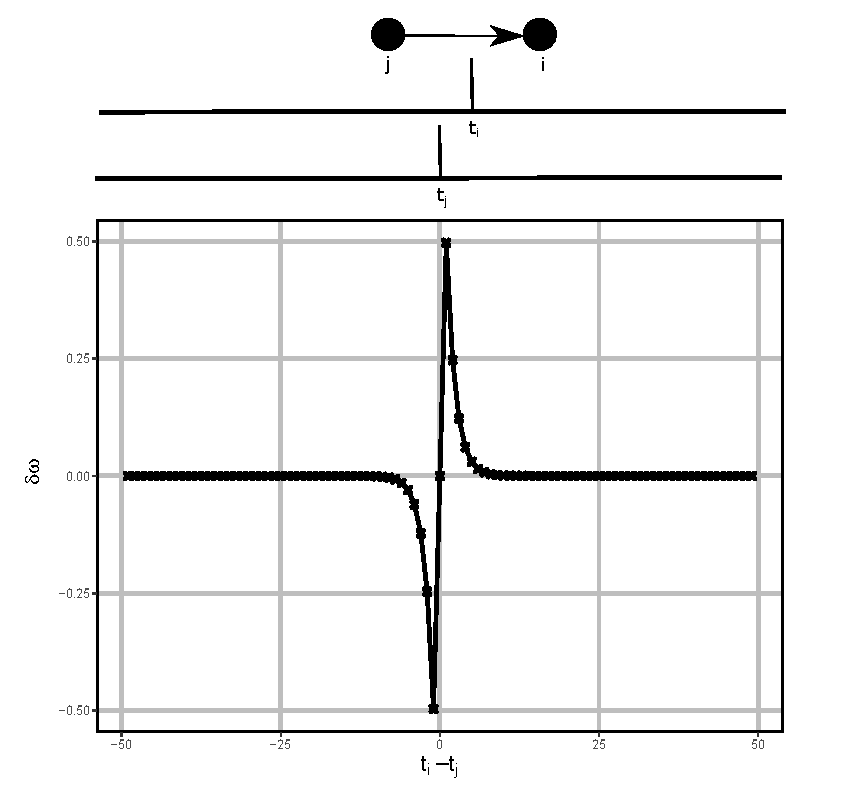
\includegraphics[width=0.8\linewidth]{fig/largesnn/STDP.eps}
	\caption{Plot showing the functional dependence of the spike-time dependent plasticity learning rule. The STDP function shows the change of synaptic weights $\Delta w$ as a function of difference in post and pre-synaptic spike-time difference.}
	\label{fig:STDP_exp1}
\end{figure}


STDP is a temporally asymmetric form of Hebbian learning induced by temporal correlations between the spike-timings of pre- and post-synaptic neurons \citep{song2000competitive}. As with other forms of synaptic plasticity, it is thought to underlie learning and memory in the brain, as well as the development and refinement of neuronal circuits during the development of the brain. With STDP, repeated pre-synaptic spike arrival, a few discrete times earlier to post-synaptic firing leads to Long Term Potentiation (LTP) of a synapse, whereas repeated spike arrival after post-synaptic spike generation leads to Long Term Depression (LTD) of the same synapse. The synaptic weight changes as a function the relative firing-time of the pre- and post-synaptic neurons, also known as the STDP learning window \citep{gerstner2002spiking}. The overall significance of STDP lies in the ability of a spiking neuron to discriminate between, and then integrate, temporally significant inputs and transforming that to meaningful output, even though the actual meaning is not strictly known by the neuron \citep{markram2011introducing}. Networks that employ STDP operates as palimpsests, \emph{i.e.} older stimuli are forgotten gradually to make room for new ones.

\citet{gerstner1996neuronal, song2000competitive} formalised the mathematical model of STDP learning as per \equationnames \ref{eq:stdp1} and \ref{eq:stdp2}. Symbols $j$ and $i$ are used to indicate pre- and post-synaptic neurons. In STDP learning, the dynamic change of weight $\Delta w$ is estimated using a learning window function $W(\cdot)$. The learning window takes historical pre-synaptic firing times $\{t_j^1 \cdots t_j^f\}$ and post-synaptic firing times $\{t_i^1\cdots t_i^g\}$ as input and calculates the LTP and LTD traces. These historical firing times are nothing but indices of a historical spike sequence. For example, a historical spike sequence $[01001011]$ can be rewritten as sequence of spike-time indices $t^f :=\{1, 4, 6, 7\}$. Exponential decay functions are a popular choice for the learning window and \equationname \ref{eq:stdp2} is a good choice of the learning window function. The $\kappa_+$ and $\kappa_-$ parameters control the maximum LTP and LTD update respectively and $\kappa_-=\kappa_+=1$ is a good choice to keep the bounds of weight update between $[-1, 1]$. From \equationname \ref{eq:stdp2}, it can be observed that the polarity of $(t^g_i-t^f_j)$ defines the polarity of $\Delta w_{ji}$. This is Hebbian model of causal relationship where synapses are rewarded positively (strengthened) for causal firing ($i$ fires later than $j$ \emph{i.e.} firing of $i$ is caused by firing of $j$) and penalised (weakened) for non-causal firing. However, \equationnames \ref{eq:stdp1} and \ref{eq:stdp2} describes a batch update scheme and requires modification for on-line learning in the SNNc. \citet{sjostrom2010spike} proposed a modified on-line STDP update rule. In the on-line setting, $\Delta w_{ji}$ is calculated every time neuron $i$ fires a spike or receives a spike from neuron $j$. \equationname \ref{eq:stdp_online} formalises the weight update rule for on-line mode. The first term in the right hand side of \equationname \ref{eq:stdp_online} corresponds to the LTP update and is calculated when neuron $i$ fires a spike at time $t$. The second term is the LTD update and is calculated when neuron $i$ receives a spike from neuron $j$ at time $t$. Both the batch and on-line formalisations of STDP learning are extended from \citep{sjostrom2010stdp} which discusses the properties of the STDP learning model extensively. \figurename \ref{fig:STDP_exp1} shows the plot of the STDP learning function where the $\Delta w$ in quadrants I and III correspond to LTP and LTD respectively.
\begin{equation}
\Delta w_{ji}:=\sum_{f}\sum_{g} W(t^g_i-t^f_j)
\label{eq:stdp1}
\end{equation}
\begin{equation}
W(s) :=
\left\{
\begin{array}{ll}
\kappa_+\exp(-s)  & \mbox{if } s > 0 \\
-\kappa_-exp(-s) & \mbox{if } s < 0
\end{array}
\right.
\label{eq:stdp2}
\end{equation}


\begin{equation}
\Delta w_{ji}(t) := \sum_f \kappa_+\exp(-(t-t_j^f))-\sum_g \kappa_- \exp(-(t-t_i^g))
\label{eq:stdp_online}
\end{equation}

It is evident from the discussion above that the STDP learning rule enhances or depletes the synaptic strength of the connections, based on the relative coincidence of the spikes. This behaviour mimics the ability of the biological neurons to encode information by detecting the occurrence of temporally close but spatially distributed input signals and thus incorporating spatio-temporal information in the model.

\subsubsection{Modified STDP in NeuCube} 
\label{subsec:mod_STDP}
\begin{figure}
	\centering
	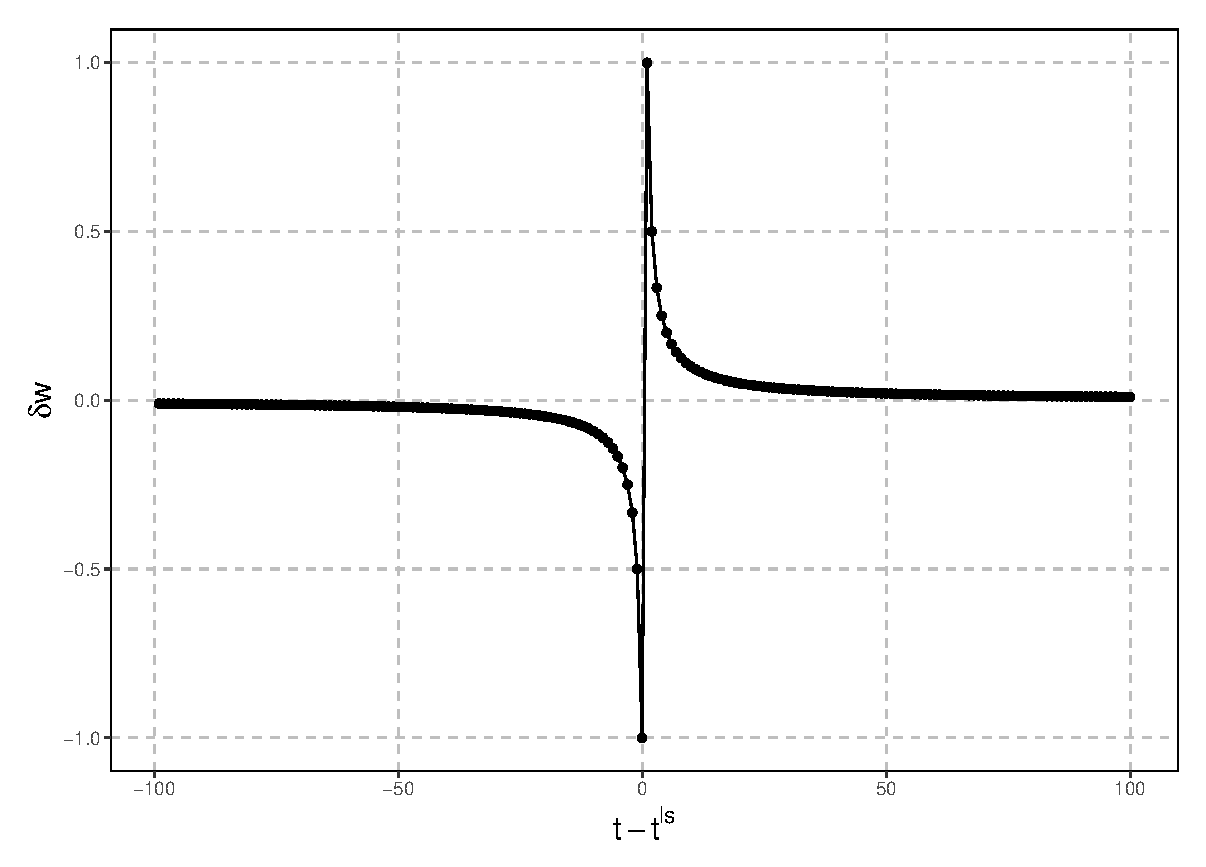
\includegraphics[width=0.8\linewidth]{fig/largesnn/mod_STDP.eps}
	\caption{Plot of modified spike-time dependent plasticity learning rule implemented in SNNc learning algorithm. The STDP function shows the change of synaptic weights $\Delta w$ as a function of difference in last and present spike-time difference.}
	\label{fig:mod_STDP_exp}
\end{figure}


The standard NeuCube implementation uses a modified form of the STDP learning algorithm. The modification mainly relates to when and which neurons are updated. The contrast between STDP and modified STDP are:

\begin{enumerate}
	\item As opposed to the STDP learning, in modified STDP learning, synaptic updates are only performed when a neuron $i$, fires a spike, and not when it receives a spike.
	\item When a neuron $i$ fires, both pre- and post-synaptic strengths are updated. The pre-synaptic connections are strengthened and post-synaptic connections are depleted. 
\end{enumerate}

The weight update rule can be formalised by \equationnames \ref{eq:mod_stdp1} and \ref{eq:mod_stdp2}, where $t^{ls}$ is the last spike time of a neuron and $t$ is the current time instance. It is quite evident that the smaller the difference between $t$ and $t^{ls}$ the more significant the weight update is. This weight update rule also implies that enhanced importance is given to faster firing rate. $\kappa_+$ and $\kappa_-$, referred to as learning rate in the NeuCube literature, control the upper and lower bound of $\Delta w$ similar to STDP. \figurename \ref{fig:mod_STDP_exp} shows the functional dependence plot of the modified STDP learning. It is quite evident from the plot that the weight update curve is very similar to the STDP weight update rule. The difference, however, lies in the functional dependence as discussed. 
   

\begin{equation}
	\Delta w_{ik}(t)=\frac{\kappa_+}{t-t^{ls}_j+1}
	\label{eq:mod_stdp1}
\end{equation}

\begin{equation}
	\Delta w_{ji}(t)=-\frac{\kappa_-}{t-t^{ls}_k+1}
	\label{eq:mod_stdp2}
\end{equation}

\begin{algorithm}
	\begin{algorithmic}[1]
		\STATE \textbf{input}: $G=\{M, C, W\}$, $D_{seq}\in \{0,1\}^{|N|\times |T|}$, $\{hyperparameters:=v_{thr}, \eta_{thr}, \kappa\}$
		\STATE \textbf{output}: $O_{seq} \in \{0, 1\}^{|M|\times |T|}$
		
		\FORALL {$t \in T$}
			\STATE initialise $C_{learn}\leftarrow\{\}$
			\FORALL {$i \in Q$}
				\STATE find firing (at $t-1$) pre-synaptic neurons, $J_i^{spk(t-1)}$
				\STATE set $C_i^{ltd}\leftarrow (J_i^{spk}, i)$
				\STATE set $C_{learn}+\leftarrow C_i^{ltd}$
				\STATE simulate neuron $i$ as per \equationname \ref{eq:SRM_neucube}
				\IF{$i$ fires}
					\STATE set $O_{seq}[i, t+1]\leftarrow 1$
					\STATE find pre-synaptic neurons, $J_i^{spk(t)}$
					\STATE set $C_i^{ltp}\leftarrow (J_i,i)$
					\STATE set $C_{learn}+\leftarrow C_i^{ltp}$
				\ENDIF
			\ENDFOR
			\FOR {$c_{ji}\in C_{learn}$}
				\STATE calculate $\Delta w_{ji}(t) \leftarrow \sum_f \kappa_+\exp(-(t-t_j^f))-\sum_g \kappa_- \exp(-(t-t_i^g))$
				\STATE update $w_{ji}+\leftarrow \Delta w_{ji}$
			\ENDFOR
		\ENDFOR
		\caption{STDP based SNNc unsupervised learning algorithm}
		\label{alg:unsup_stdp}
	\end{algorithmic}
\end{algorithm}

\subsection{Formal Description of SNNc Unsupervised Learning Algorithm}
\label{sec:neucube_snnc_learning}
\begin{algorithm}
	\begin{algorithmic}[1]
		\STATE \textbf{input}: $G=\{M, C, W\}$, $D_{seq}\in \{0,1\}^{|N|\times |T|}$, $\{hyperparameters:=v_{thr}, \eta_{thr}, \kappa\}$
		\STATE \textbf{output}: $O_{seq} \in \{0, 1\}^{|M|\times |T|}$
		
		\FORALL {$t \in T$}
		\STATE initialise $C_{learn}\leftarrow\{\}$
		\FORALL {$i \in Q$}
		\STATE find firing (at $t-1$) pre-synaptic neurons, $J_i^{spk(t-1)}$
		\STATE simulate neuron $i$ as per \equationname \ref{eq:SRM_neucube}
		\IF {$i$ fires}
		\STATE set $O_{seq}[i, t+1]\leftarrow 1$
		\STATE find pre- and post-synaptic neurons $J_i^{spk(t)}$ and $K_i^{spk(t)}$
		\STATE set $C_i^{ltp}\leftarrow (J_i^{spk(t)}, i)$ and $C_i^{ltd}\leftarrow (i, K_i^{spk})$
		\STATE set $C_{learn}+\leftarrow C_i^{ltp}$ and $C_{learn}+\leftarrow C_i^{ltd}$
		\ENDIF
		\ENDFOR
		\FOR{$\{c_{ji}, c_{ik}\} \in C_{learn}$}
		\STATE calculate $\Delta w_{ji}\leftarrow \frac{\kappa}{t-t_j^{ls}+1}$ and $\Delta w_{ik}\leftarrow -\frac{\kappa}{t-t_k^{ls}+1}$
		\STATE update $w_{ji}+\leftarrow \Delta w_{ji}$ and $w_{ik}+\leftarrow \Delta w_{ik}$
		\ENDFOR
		\ENDFOR
		\caption{Modified STDP based SNNc unsupervised learning algorithm}
		\label{alg:unsup_mod_stdp}
	\end{algorithmic}
\end{algorithm}

A classical implementation of the SNNc unsupervised learning algorithm is formally presented in \algorithmname \ref{alg:unsup_mod_stdp}. This algorithm uses the modified STDP learning described in Section \ref{subsec:mod_STDP}. The goal of the learning algorithm is to continuously input data sequence $D_{seq}$ in the form of spikes and simulate the network $G$ in a way that the synaptic strengths $W$ of the network are updated over time $T$ to learn poly-synchronous relationships across space and time. The hyperparameters for neuron simulation ($v_{thr}, \eta_{thr}$) and learning ($\kappa$) are also input into the learning algorithm. At the end of the simulation, the algorithm outputs the  spike sequence $O_{seq}$. The simulation of G is performed at every time instance $t \in T$ and is described within the loop between line $3$ and $19$ in \algorithmname \ref{alg:unsup_mod_stdp}. At every time instance, an empty variable $C_{learn}$ is initialised, which stores over the subsequent steps, a subset of connection identities ($C_{learn}\subset C$) for the synaptic strength updates. The simulation is then performed in two subsequent phases. In the first phase (line $5$ to line $14$), all the spiking neurons $Q$ are simulated based on the spiking neuron model. In NeuCube, the neuron simulations are done following \equationname \ref{eq:SRM_neucube}. In NeuCube, pre- ($J_i^{spk(t)}, i$) and post-synaptic ($i, K_i^{spk(t)}$) connections of the spiking neurons that fire at time instance $t$ are candidates for weight evolution. These connections are stored in $C_{learn}$ for update. The second step (line $15$ to line $18$) is the learning stage. During the learning stage, the connections $C_{learn}$ are updated according to the learning rule, which in case of \algorithmname $\ref{alg:unsup_mod_stdp}$ is the modified STDP learning rule. In addition, \algorithmname \ref{alg:unsup_stdp} also presented the SNNc unsupervised learning algorithm using the canonical STDP learning rule described in Section \ref{subsec:STDP}. A careful comparison between the two algorithms reveal that the synaptic strength update in modified STDP is drastically different from canonical STDP in regards to when and what synapses are updated.    

\subsubsection{Considerations for Parallelisation}
Neural networks are generally considered as a massively parallel problem, \emph{i.e.}, the computations are simultaneous rather than sequential in layers of a typical neural network. Therefore, the divide and conquer type of parallelisation construct can be very easily achieved in neural networks by using the map and reduce paradigm of functional programming. However, by observing the characteristics of the SNNc learning algorithm, there does not seem to be a clear parallelisation approach. This is caused by the recurrence present as the output of the neurons in the SNNc layer, in the form of spike sequences which are recurrently fed back to other neurons creating a neuron level dependency over space and time. Therefore, although it is very tempting to merge the learning step and the neuron simulation step across the spiking neurons together, the asynchronous nature of the updates deems it an extremely hard parallelisation problem. The system clock driven computational simulation at the moment is clearly different from the clock precise parallelised scheme in the brain.    

\section{Analysis of the Data Structure Representations of SNNc} 
In this Section, focus of attention will be on the SNNc network structure representation $G$ in light of \algorithmname \ref{alg:unsup_mod_stdp}. The overall objective of the network structure representation analysis is guided by the objective to improve the computation and storage load of the algorithm as the unsupervised learning mechanism evolves the network over time. This work specifically looks into the storage and time complexity of the algorithm with increasing numbers of neurons in the network. During the iterative simulation process, the connections and the weights of the network are accessed very frequently. Parts of the SNNc network are accessed specifically in lines $6, 10-12$ and $15-17$. The access to the network is theoretically a search operation within the search space $C$ for information on specific neuron identities. In particular, the algorithm needs to access the immediate neighbours of a given neuron $i$. These are the pre- and post-synaptic neurons $J_i^{spk}$ and $K_i^{spk}$. A data structure that is used for representing the network must, therefore, provide fast accessibility of neighbouring nodes. As an additional constraint, the present work focuses on the algorithmic implementation of a general purpose von-Neumann architecture computer (as opposed to the implementation on a neuromorphic hardware \citep{scott2015thesis} setup), designed for  commodity consumption. Therefore, storage space and computing capacity are of course constrained and an optimum data structure representation should be storage- and time-efficient. For the current experiments, a general purpose PC running a 64 bit Windows 7 enterprise operating system was used; one that had 16GB RAM, Intel Core i5 processor with 3.20 GHz clock speed. The implementations of \algorithmname \ref{alg:unsup_mod_stdp} was done in Matlab version R2014b.

In the Matlab based prototype and testing version of NeuCube, an adjacency matrix was used to store the connection structure $C$. According to graph theory, an adjacency matrix is defined as a square matrix $C$ of order $M$ (number of neurons) where 1 represents an existing edge between the two vertex indices. The edges correspond to the connections, and the vertices are the neuronal unique identifiers. In the present implementation, a second adjacency matrix is needed to store the weights $W$ in order to avoid confusion between the existence of an edge and the weight values themselves. \figurename \ref{fig:adj_mat} shows an example of an adjacency matrix. Since all values in an adjacency matrix can be directly accessed by using the corresponding neuron IDs as indices, this data structure is extremely fast. However, due to the nature of storing all relations between vertices, the storage had grown at a squared rate, and it also showed to be the most storage demanding option when compared to other data structures. 
\begin{figure}
	\centering
	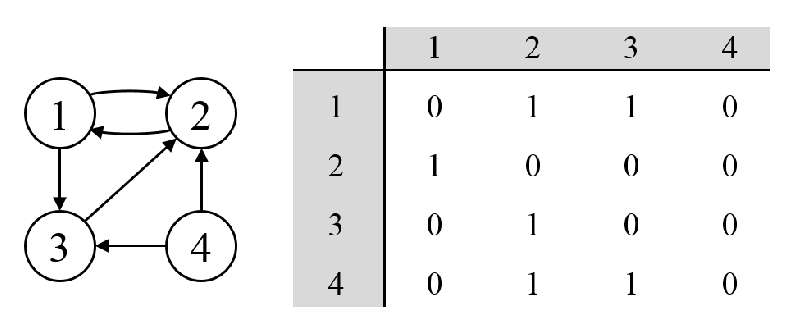
\includegraphics[width=0.5\linewidth]{fig/largesnn/adj_matrix.eps}
	\caption{Example of the adjacency matrix representation.}
	\label{fig:adj_mat}
\end{figure}

The second option that was investigated was an edge-weight table. An edge-weight table stores the connection and their weights in a simple look-up table with each row containing a pair of neuron indices (identities) $i$ and $j$, and the weight of the connection between them, as shown in \figurename \ref{fig:ijv_tab}. This edge-weight table used far less storage than the adjacency matrix; however, it was also considerably slower, because in order to access a connection between a pair of neurons, the whole table had to be searched, which meant an average time complexity of $O(\frac{1}{2}c)$. Ordering the table by neuron $i$ to use it as an index could to some extent alleviate the problem for finding post-synaptic neurons, but not for pre-synaptic neurons, since in that case only neuron $j$ was given. Therefore, this data structure is sub-optimal in regards to computation time especially in case of larger networks.

\begin{figure}
	\centering
	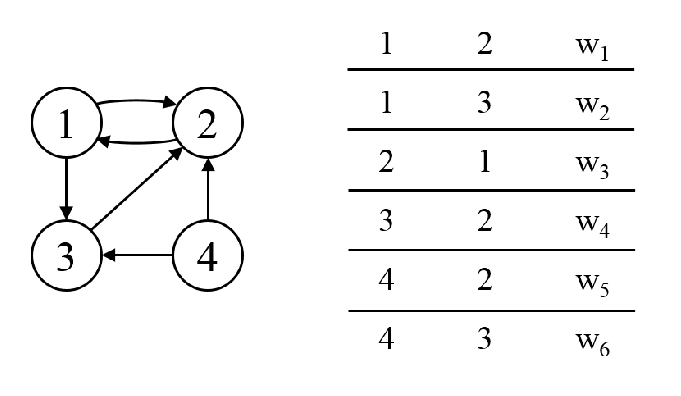
\includegraphics[width=7cm]{fig/largesnn/ijv_table.eps}
	\caption{Example of the edge-weight table representation.}
	\label{fig:ijv_tab}
\end{figure}

The third data structure was an adjacency forward list. In graph theory, this is a list of vertices in which each entry contains a sub-list of neighbouring vertices. An example for an adjacency forward list is depicted in \figurename \ref{fig:adj_list}. In terms of storage space, the adjacency list, like the edge-weight table, is considerably smaller than the adjacency matrix as it only stores the connections. Compared to the edge-weight table, the adjacency forward list saves space by listing all neurons connected to neuron $i$ in an indexed list (the index being neuron $i$) instead of repeating the index for every connection. However, for \algorithmname \ref{alg:unsup_mod_stdp}, a second adjacency forward list was needed to store the weight values of the connections, which is why this data structure uses slightly more storage space than the edge-weight table in the experiments. In terms of temporal performance, the adjacency forward list was also very similar to the edge-weight table in that it was faster to access post-synaptic connections due to indexing than looking up pre-synaptic connections where all sub-lists had to be searched. However, the indexing mechanism of the adjacency forward list provides a significantly faster look-up of post-synaptic connections than the edge-weight table. For these reasons, the adjacency forward list is overall expected to scale up best for a larger number of neurons, compared to the edge-weight table and the adjacency matrix.

\begin{figure}
	\centering
	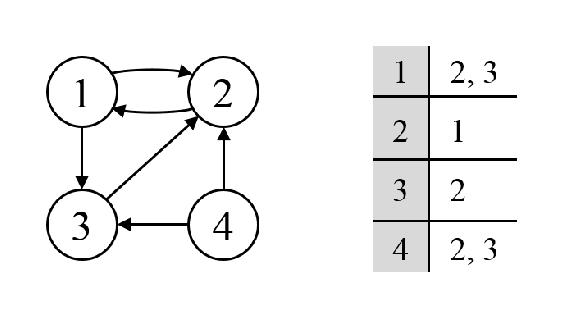
\includegraphics[width=6.2cm]{fig/largesnn/adj_list.eps}
	\caption{Example of the adjacency forward list representation.}
	\label{fig:adj_list}
\end{figure}

Taking into consideration that the adjacency forward list is a very storage-efficient data structure and that its main bottleneck for temporal performance is the look-up of pre-synaptic indices, a decision was made to add a second adjacency list called an adjacency backward list to the structure to represent the connections from the opposite perspective, thus making the neuron at the end of the connection (neuron $j$) the index of this second list. A schema of this approach is shown in \figurename \ref{fig:fw_bw_adj_list}. This “backwards” indexing mechanism caused a significant decrease of the algorithm's execution time, because it effectively reduced the time complexity of the data structure to $O(1)$ for finding the right pre-synaptic and post-synaptic indices. In comparison with the other data structures, the adjacency forward-backward list was now the best alternative for representing the SNNc network. \tablename \ref{tab:complexity} gives a comparative overview of the theoretical complexities in regards to time and storage with the different data structures discussed here. The complexities are measured by $n$ and $c$ referring to the neuron count and connection count respectively. The relationship between $n$ and $c$ can be represented by $c=\alpha\times n^2$, where $\alpha\in [0, 1]$ is the degree of sparseness. All of the present experiments have used $\alpha=0.02$. 

\begin{figure}
	\centering
	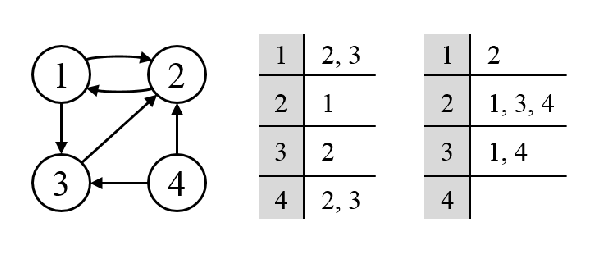
\includegraphics[width=7.8cm]{fig/largesnn/adj_bw_list.eps}
	\caption{Example of the adjacency forward-backward list representation.}
	\label{fig:fw_bw_adj_list}
\end{figure}

\begin{table}
	\centering
	\caption{Comparison of time and storage complexity for different data structures.}
	\label{tab:complexity}
	\resizebox{\textwidth}{!}{\begin{tabular}{@{}|l|c|c|c|c|c|@{}}
		\toprule \toprule
		\multirow{2}{*}{data structure} & \multicolumn{1}{c|}{\multirow{2}{*}{connection type}} & \multicolumn{3}{c|}{time} & \multirow{2}{*}{storage} \\ \cmidrule(lr){3-5}
		& \multicolumn{1}{c|}{} & \multicolumn{1}{c|}{worst} & average & best &  \\ \midrule
		adjacency matrix & all & \multicolumn{3}{c|}{$O(1)$} & \multicolumn{1}{c|}{$S(n^2)$} \\ \midrule
		edge-weight table & all & $O(c)$ & $O(\frac{1}{2}c)$ & $O(1)$ & $S(c)$ \\ \midrule
		\multirow{2}{*}{adjacency forward list} & pre-synaptic & \multicolumn{1}{c|}{$O(c)$} & $O(\frac{1}{2}c)$ & $O(1)$ & \multicolumn{1}{c|}{\multirow{2}{*}{$S(2\times c)$}} \\ \cmidrule(lr){2-5}
		& post-synaptic & \multicolumn{3}{c|}{$O(1)$} & \multicolumn{1}{c|}{} \\ \midrule
		adjacency forward-backward list & all & \multicolumn{3}{c|}{$O(1)$} & \multicolumn{1}{c|}{$S(3\times c)$} \\ \bottomrule \bottomrule
	\end{tabular}}
\end{table}

The findings from the theoretical analysis of the structures' complexity could be verified through the present experimental results. For the experiments, a benchmark EEG dataset was used. The dataset consisted of EEG data measuring brain signals during a task of wrist movement. The wrist movements were categorised into upward, downward, and central directions. This task was performed on a single subject and EEG data was sampled from $14$ channels at a sampling rate of $128$ Hz while the subject performed the task. $20$ independent trials of one second duration were collected while the subject performed each movement task. $14$ of the $1485$ neurons in the reservoir were randomly chosen as input neurons for the EEG channels. A network with a highly sparse connectivity ($\approx 2\%$ of all possible connections) was initialised randomly for every experiment. The value of two per cent was chosen because this was the average amount of connections used typically during experiments.

\figurename \ref{fig:storage_comp} shows the comparison of storage required in megabytes by each of the data structures. The graph itself is dependent on the number of neurons in the SNNc (between $0$ and $70,000$ for the storage, and between $500$ and $3,500$ for the execution time). When it was decided that the number of neurons should be increased further, all values above $80,000$ neurons for the adjacency matrix and above $120,000$ neurons for the sparse matrix had to be excluded, due to the above discussed technical restrictions in the experimental setup. In addition, it became difficult to distinguish between the curves, especially in the lower regions of the graph.

\begin{figure}
	\centering
	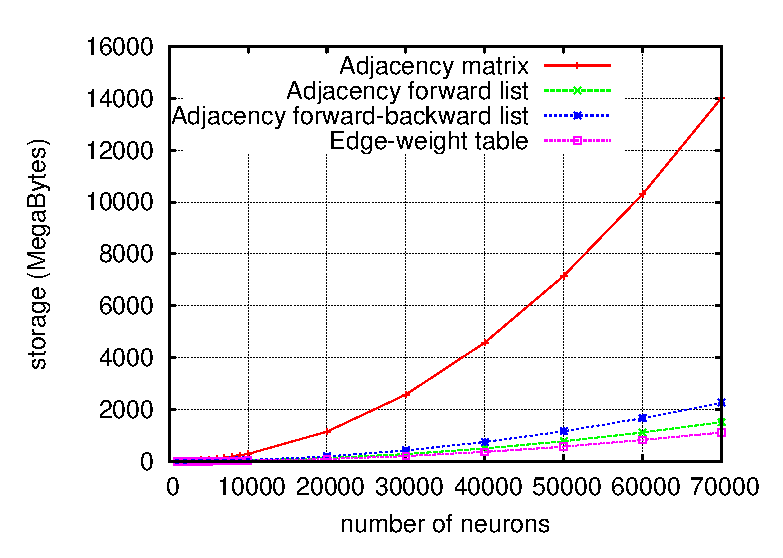
\includegraphics[width=0.8\linewidth]{fig/largesnn/storage.eps}
	\caption{Storage space comparison of different data structures with increasing number of neurons.}
	\label{fig:storage_comp}
\end{figure}

\begin{figure}
	\centering
	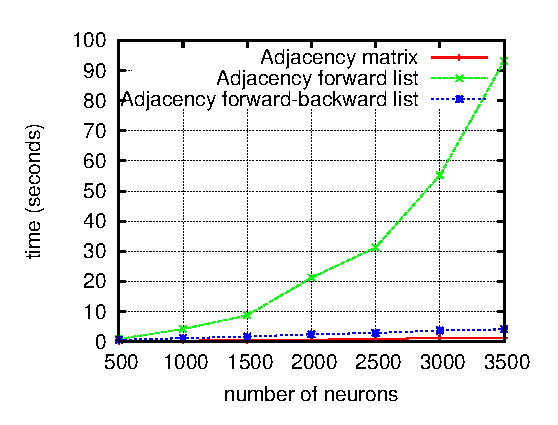
\includegraphics[width=0.8\linewidth]{fig/largesnn/time.eps}
	\caption{Execution time comparison of different data structures with increasing number of neurons.}
	\label{fig:time_comp}
\end{figure}

It is clearly visible that the adjacency matrix has the steepest increase of storage space needed. The other three data structures are relatively similar in their development, with the edge-weight table growing slowest. It was interesting to see that the curve of the sparse matrix was very close to the one of the adjacency list, which indicates that the internal representation of a sparse matrix in Matlab is similar to an adjacency list. \figurename \ref{fig:time_comp} shows the results of comparing the execution time of the data structures. For the comparison of execution times, the curve of the edge-weight table showed its disadvantage as it increases near exponentially. Thus, another graph representation without the edge-weight table was created. This showed that the adjacency list was considerably slower than the matrices and the adjacency backwards list.

These experimental results verify the previous theoretical analysis. The most promising data structure for representing an SNNc network having a large number of neurons in the NeuCube SNN is the adjacency list with backwards indexing due to its constant complexity in terms of execution time of the algorithm, and linear storage growth with increasing connection density.


\subsection{Large-scale Unsupervised Learning of SNNc Using the Adjacency Forward-backward List}

\begin{figure}
	\centering
	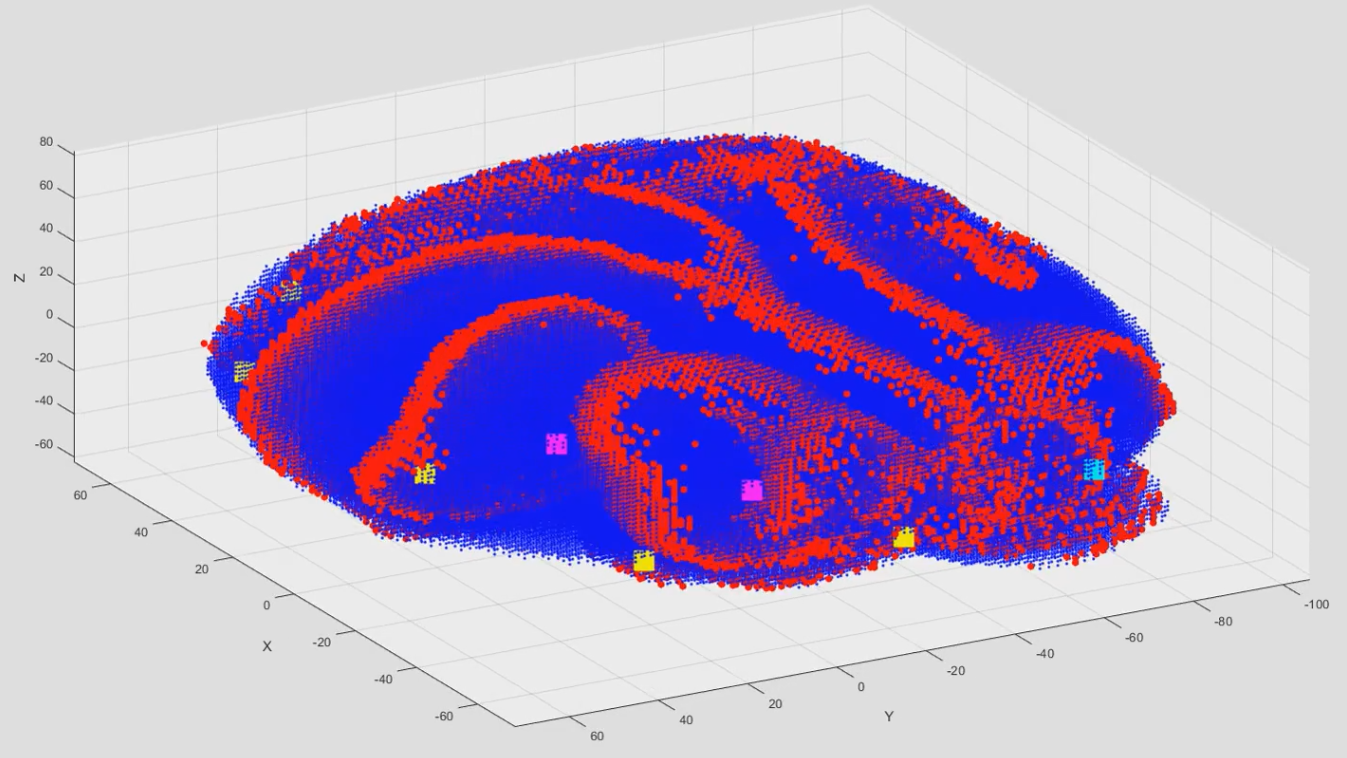
\includegraphics[width=0.8\linewidth]{fig/largesnn/spike_simulation.png}
	\caption{Snapshot of the spike activity at a time instant inside the SNNc.}
	\label{fig:spike_simulation}
\end{figure}

\begin{figure}
	\centering
	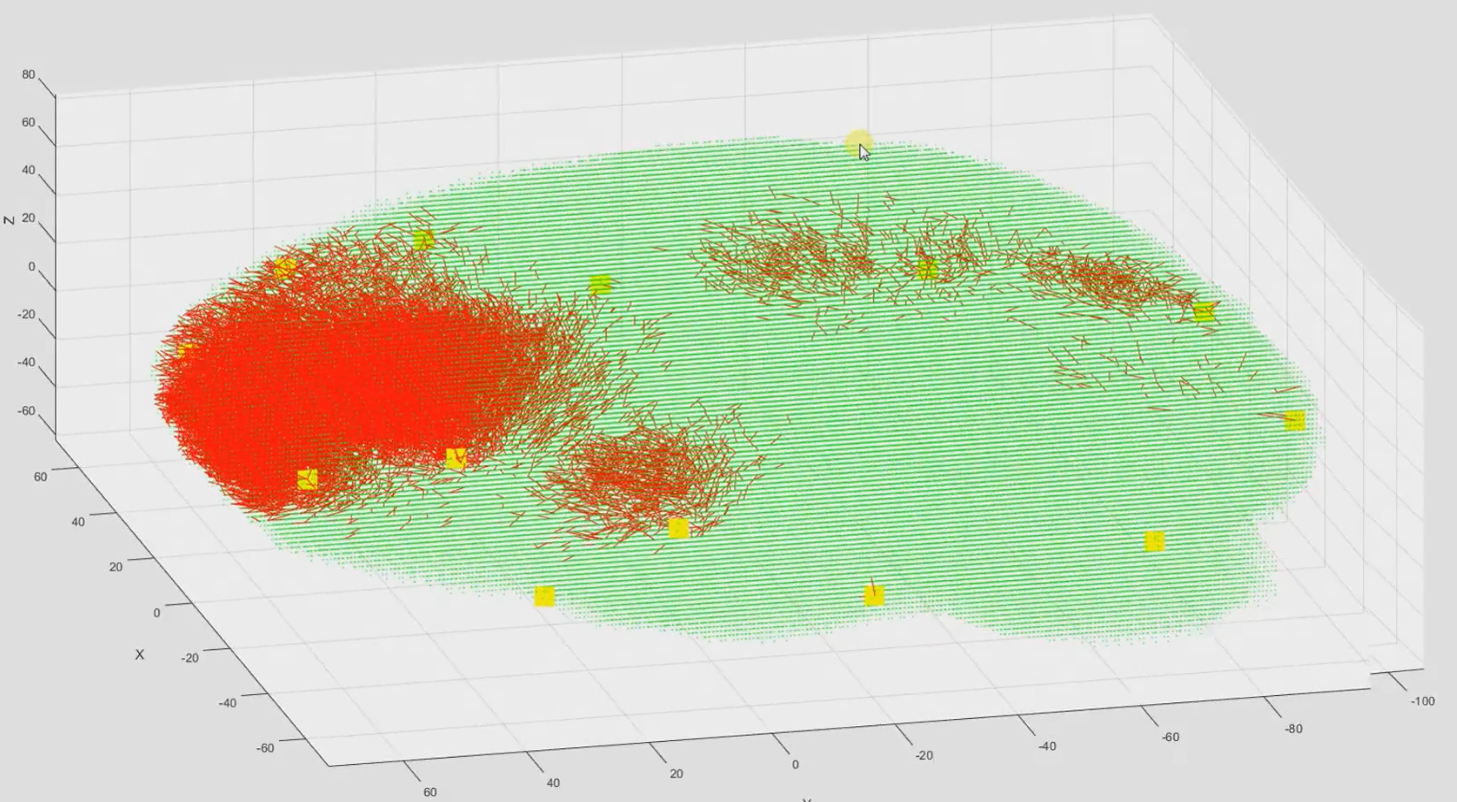
\includegraphics[width=0.8\linewidth]{fig/largesnn/connection_simulation.png}
	\caption{Strongest connections learned by the SNNc at the end of SNNc simulation.}
	\label{fig:connection_simulation}
\end{figure}

As a conclusion of the current experimental results, it seemed evident that the adjacency forward-backward list data structure representation is the most economic in regards to storage and temporal complexity. To further demonstrate this, the NeuCube SNNc learning algorithm in Matlab capable of using the adjacency forward-backward list data structure was implemented (see Appendix \ref{chap:app_SNNc_unsupervised} for the Matlab programme). In order to test the efficiency of the implementation on a much larger scale, \algorithmname \ref{alg:unsup_mod_stdp} was run on a SNNc consisting of $241,606$ neurons taking the same EEG input data described earlier. The SNNc was simulated to mimic a brain with neural cells in the order of $10^6$ and connections in the order of $10^{10}$. The spatial coordinates of the neurons were obtained from the xjView \citep{cui2011xjview} software and resembled the spatial distribution of the human brain based on the MNI coordinate system. \figurename \ref{fig:spike_simulation} shows a snapshot of spiking patterns at a certain time instance during the unsupervised learning simulation. The ripple like behaviour of the liquid state within the SNNc can be clearly observed in the network. The ripple effect in the SNNc is of course clearly visible in a dynamic simulation environment. \figurename \ref{fig:connection_simulation} shows the strongest connections formed in the brain-like network as a result of the unsupervised learning.

\section{Considerations for Modularity and Heterogeneity: Towards Graph Based Software Design of SNNc}
In the last Section, the considerations of scalability in regards to the size of the SNNc was discussed. At this point, it is critical to mention that apart from the large size, biological brains are considerably modular and heterogeneous. The theory of modularity suggests that there are functionally specialised regions in the brain that are domain specific for different cognitive processes. The brain is often represented as a network of interconnected, dynamically interacting elements. Cognitive processes are thought to result from the integration of neuronal processing distributed across these complex networks at different temporal and spatial scales. Several graph theory based methods \citep{sporns2016modular, nicolini2016modular} have been proposed in analysing the modularity and heterogeneity in the brain.

The idea of modularity and heterogeneity is of major importance for the neuromorphic inspirations of the SNNc architecture design. Heterogeneity and modularity is observed not only in the brain but is quite prevalent in a broad range of networks, such as groups in social networks, ensembles of interacting proteins or coregulated genes in cellular network. These clusters or groups of items have homogeneous property behaviours within the group, and vary considerably between the groups across the network. 

The objective of this Section was to design algorithmic or implementation improvements to facilitate heterogeneity and modularity in the SNNc. Let us revisit the implementation of unsupervised learning algorithms (see Appendix \ref{chap:app_SNNc_unsupervised}). The functional style of implementation constrains the ability to inject heterogeneity into the network, especially if one considers designing networks with varieties of neurons, synapses, learning behaviour etc. 

The basic concept behind the template method design pattern is relatively simple. Generally abstract classes are created representing necessary steps for a general algorithm operation. An instantiation of the template (class) then implements these steps with necessary extension. In \algorithmname \ref{alg:unsup_mod_stdp}, the network $G$ is represented by the tuple $<M, C, W>$. $M$ is a list of neuron identifiers and serves no purpose other than storing the identifiers. The code for neuron simulation is integrated within the network simulation programme and is independently treated compared to $M$. Additionally, weights are modelled independently of the connections in \algorithmname \ref{alg:unsup_mod_stdp}. 

In order to overcome these shortcomings, the SNNc network in the graph based design is constructed as a directed graph data structure. The graph based architecture that was designed is summarised in the UML class diagram shown in \figurename \ref{fig:class_diagram}. The graph $G=<V, E>$ is made of vertices $V=\{v_1,v_2, \cdots, v_m\}$ and edges $E=\{e_1, e_2,\cdots, e_c\}$. The class SNNc is designed at the network level of abstraction, where behaviours and operations are performed on the whole or part of the network. Some operations on the network are $initialiseNetwork()$: used to initialise the SNNc network. Several algorithms can be implemented as part of the SNNc class; $learnNetwork()$: Method to perform unsupervised learning on the SNNc network. This method should be used to handle the synchronisation and broadcasting of the data in the form of spikes across the network; $visualiseNetwork()$: is used to visualise the dynamic and static states of the network. The output of this method are similar to the ones shown in \figurenames \ref{fig:connection_simulation} and \ref{fig:spike_simulation}. The vertices and edges forming the SNNc graph are designed to be modelled individually. Personalised models of vertices and edges ensures the flexibility of implementing varying degrees of heterogeneity in the network through encapsulation and polymorphism of the objects.  

A vertex in graph $G$ is modelled as an object with the following properties:
\begin{enumerate}
	\item ID: Stores the unique identification of a vertex.
	\item Location: Stores the spatial location of the vertex in the 2D/3D space.
	\item Neuron: Refers to an instance of a suitable neuron model. The Neuron object is modelled as an instantiation of the $GenericNeuron$ class which can morph into either input or spiking neurons. A couple of implementations of spiking neuron models that inherits from the $GenericNeuron$ are shown as $LIFNeuron$ and $IzhikevichNeuron$. Each of the spiking neurons are initialised by the $init()$ method and simulated over time using the $simulate()$ method.  It is evident that the realisation of any neuron models or even newer behaviours in the existing neuron models can be achieved without much effort through this modular design. 
\end{enumerate}
An edge in graph $G$ consists of the following properties:
\begin{enumerate}
	\item ID: Stores the unique identification of an edge.
	\item fromVertexID: Stores the source vertex ID of the edge.
	\item toVertexID: Stores the destination vertex ID of the edge.
	\item synapse: Refers to an instance of a suitable synapse model implementation. An example synapse model is described in class $Synapse$. The primary behaviour of the synapse is controlled $updateSynapse()$ method. This method modifies the synaptic strength (weight) using learning rules implemented as static methods.  
\end{enumerate}

Overall to inject modularity and variety in the SNNc, the architecture has been designed in hierarchical layers of abstraction in a top-down manner. At the highest layer of abstraction, the SNNc network has been designed only at network level, keeping the vertex and edge level implementations abstract. In the next layer of hierarchy, the individual vertices and edges are modelled and drills down further into individual neuron models, learning behaviour and so on. Implementing the architecture this way also allows a user to configure the SNNc at varying degrees of generality.     
\begin{sidewaysfigure}
	\centering
	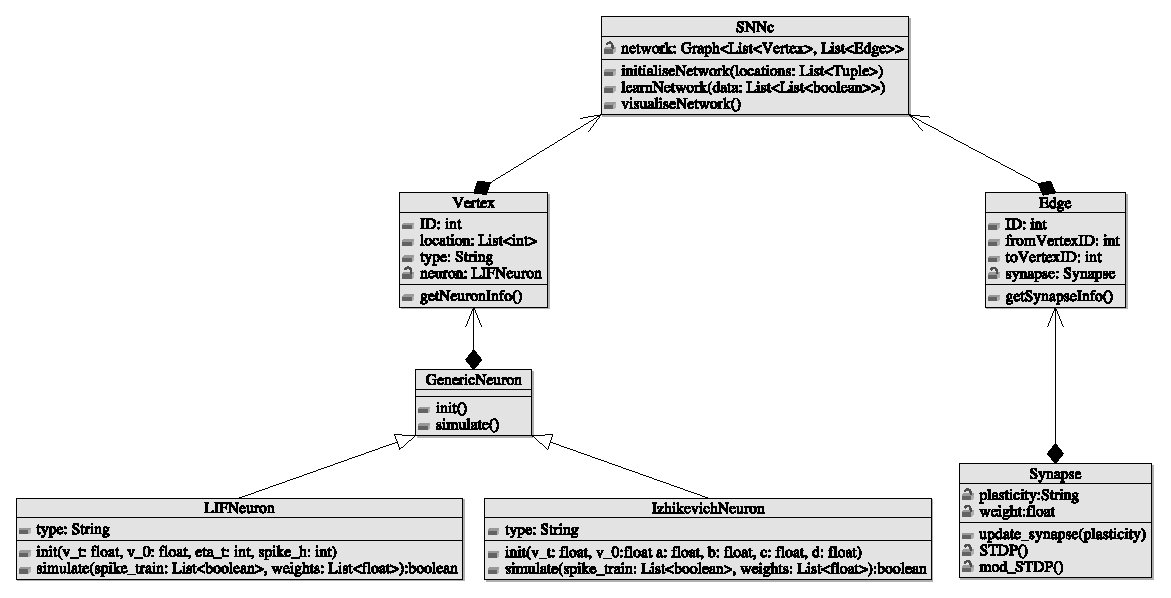
\includegraphics[width=0.8\linewidth]{fig/largesnn/class_diagram.eps}
	\caption{UML Class diagram of the template based object-oriented architecture of the SNNc. This architecture should be considered an example architecture for incorporating modularity. A python implementation of the SNNc following this architecture is presented in Appendix \ref{chap:app_SNNc_unsupervised}.}
	\label{fig:class_diagram}
\end{sidewaysfigure}

\section{Summary and Conclusion}
In this Chapter, the discussions have primarily revolved around the implementation aspects of the SNNc. This Chapter began by contemplating the discrepancy between a biological brain and a computer. The discrepancies formed the basis of the challenges that arises in developing human brain-like computation algorithms in computers. Then, there was a presentation of an in-depth formalisation, discussion and analysis of the several components of the SNNc architecture and unsupervised learning algorithms in NeuCube. This discussion paves the pathway for analysing the data structure representations of the SNNc network with respect to scalability and heterogeneity. During this discussion, it was shown how the network representation plays a decisive role in large scale implementations, especially balancing the storage and execution time. The importance of modularity and heterogeneity in SNNc was further discussed as well as a proposal put forward for a hierarchical template pattern-based software architecture for realising such a goal.


\pagebreak
\section{Contributions and Publications}
\begin{tcolorbox}[colback=black!5,colframe=black!40!black,title=Contributions]
	\itshape
	\begin{enumerate}
		\item There were qualitative comparisons of the contrasting characteristics of a biological brain and a computer.
		\item In-depth descriptions about the SNNc layer of the NeuCube architecture were made. This included SNNc network initialisation, simulation and learning with formalisation of the unsupervised learning algorithm.
		\item An analyses of the SNNc network storage architecture and data structure was presented in the light of large scale simulation of the SNNc.
		\item A template pattern based software design architecture of SNNc to incorporate modularity and heterogeneity in the SNNc was proposed and implemented.   
	\end{enumerate}

\end{tcolorbox}

\begin{tcolorbox}[colback=black!5,colframe=black!40!black,title=Publications]
	\begin{enumerate}
		\item Abbott, A., \textbf{Sengupta, N.}, \& Kasabov, N. (2016, July). Which method to use for optimal structure and function representation of large spiking neural networks: A case study on the NeuCube architecture. In Neural Networks (IJCNN), 2016 International Joint Conference on (pp. 1367-1372). IEEE.
	\end{enumerate}
\end{tcolorbox}



